-------------------------------------------------------------------------------
% 
\chapter{Knowledge Acquisition Approach}
%-------------------------------------------------------------------------------

This chapter defines the terms, formal structure and steps that form our 
proposed KA approach. First it introduces the general architecture and 
interaction loop that defines the sequence of interactions and steps
involved in the process(\autoref{section:Architecture}). In the second part, it
formalizes the upper ontology and logical constructs required for the KA 
approach (\autoref{section:kb}). After that, each of the crucial steps is 
described in more detail through examples and additions to the core logical 
structure defined earlier.

To make it easier to explain, formalize and understand the proposed approach 
for automated knowledge acquisition with prior knowledge, user context and 
conversational crowdsourcing, we will guide the explanations and formalizations
through an example KA conversation depicted in tables \ref{tab:conversation1}
and \ref{tab:conversation2}.

%Define step counter for chat steps
\newcounter{stepno}
\newcommand{\step}[1]{\refstepcounter{stepno}\label{#1}}

\begin{table}[h!]
\centering
\caption{Minimal example of Curious Cat and user interaction.}
\label{tab:conversation1}
\begin{tabular}{|c|l|l|}
	\hline
	\multirow{2}{2em}{Step num.} & \multicolumn{2}{c|}{Interaction}\\\cline{2-3}
	& \multicolumn{1}{c|}{Curious Cat} & User1 \\
	\hline
	\step{step:where} 1& \makecell[l]{Where are we? \\Are we at Joe's Pizza restaurant?} & Yes.\\
    \hline
	\step{step:kind} 2 & \makecell[l]{We've never been here before.\\ What kind of place this is?} & Restaurant.\\
    \hline
    \step{step:wifi} 3 & Does Joe's Pizza have Wi-Fi? & Yes. \\
    \hline
    \step{step:fast} 4 & Is it fast enough to make Skype calls? & I don't know.\\
    \hline
    \step{step:menu} 5 & What's on the menu in Joe's Pizza? & Pizzas.\\
	\hline
    \multicolumn{3}{|c|}{...Some time passes while the user eats...}\\
	\hline
	6 & What did you order? & A car. \\
	\hline
	7 & \makecell[l]{I've never heard of food called 'car' before. \\ Are you sure it's a type of food?} & No. \\
	\hline
	8 & What did you order then? & Pizza Deluxe \\
	\hline
	9 & \makecell[l]{I've never heard of 'Pizza Deluxe' before.\\What kind of thing is it?} & Pizza. \\
	\hline 
\end{tabular}
\end{table}

When the system is convesing with the user, it uses all the knowledge gathered 
in prior conversations, other user's conversations and also this conversation, 
and is able to use it to further generate new comments and related questions. 
This is evident in the interaction step number 4 in \autoref{tab:conversation1}. 
At the same time, or later, when some other user is in a similar context, 
the knowledge can be double checked with another user, as shown in 
\autoref{tab:conversation2}. Based on the votes (confirmations or rejections) 
from the crowd (other users), the system can decide whether to believe the new 
knowledge in general, or only when it interacts with this particular user.
This is explained in more detail in section \hl{ref}.

\begin{table}[h!]
\centering
\caption{Minimal example of Truth checking interaction with the help of 
	crowdsourcing.}
\label{tab:conversation2}
\begin{tabular}{|c|l|l|}
	\hline
	\multirow{2}{2em}{Step num.} & \multicolumn{2}{c|}{Interaction}\\\cline{2-3}
	& \multicolumn{1}{c|}{Curious Cat} & User2 \\
	\hline
	10 & \makecell[l]{Where are we? \\Are we at Joe's Pizza restaurant?} & Yes.\\
    \hline
	11 & \makecell[l]{We've never been here before.\\ What kind of place this is?} & Restaurant.\\
    \hline
\end{tabular}
\end{table}

The resulting implementation (described at the end in 
\autoref{chapter:implementation}) of the described approach, named Curious Cat 
has a multi objective goal, KA is the primary goal, while having an intelligent 
assistant and a conversational agent are secondary goals. The aim is to perform
knowledge acquisition effortlessly and accurately as a side effect, while having
a conversation about concepts which have some connection to the user.
At the same time, the approach allows the system (or the user) to follow the 
links in the conversation to other connected topics, covering and collecting
more knowledge. For illustration see the example conversation sketch in 
]hl{Table I}, where the topic changes from a specific restaurant to a type of 
dish.

\section{Architecture}
\label{section:Architecture}
The proposed KA system consists of multiple interconnected technologies and 
functionalities which we grouped into logical modules according to
the problems they are solving (as also defined in \autoref{chapter:background}). 
This was done in order to minimize the complexity, improve the maintenance 
costs and allowing switching the implementations of separate sub-modules. 
Additionally such logical grouping increases the explainability and general
understanding of the system.

\begin{figure}[htb]
	\centering
		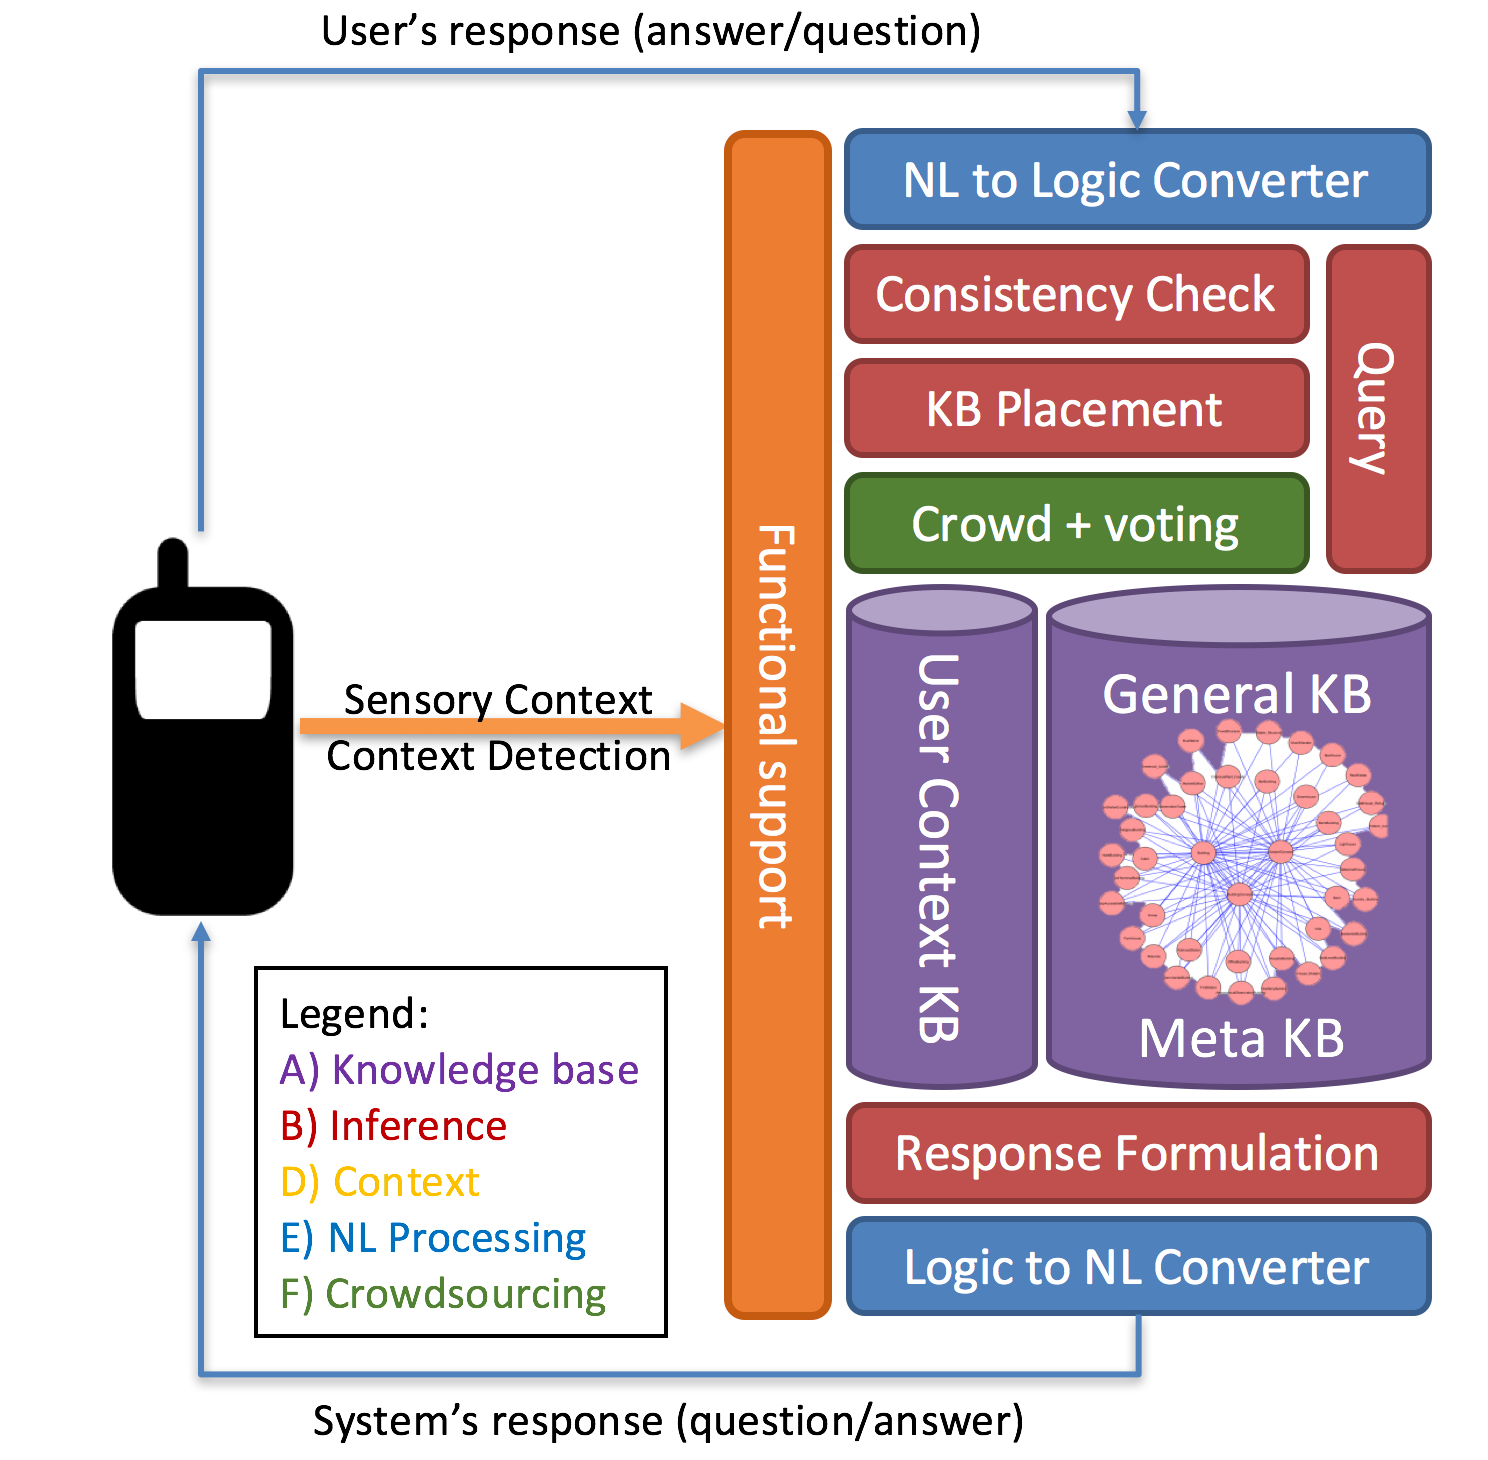
\includegraphics[width=0.9\textwidth]{figures/architecture.png}
	\caption{General Architecture of the KA system, with an interaction loop
			 presented as arrows.}
	\label{fig:Architecture}
\end{figure}

On \autoref{fig:Architecture} these modules are represented with the boxes,
and their functionality groups are presented with the colors (see the figure
legend). Arrows represent the interaction and workflow order and initiation 
(the interaction is initiated/triggered from the origin of the arrow).

We can see that the central core of the
system is the knowledge base (modules marked in purple and letter A). The 
knowledge base consists of \emph{Upper Ontology} gluing everything together, 
\emph{Common Sense Knowledge} to be able to "understand" user's world and check
the answers for consistency, \emph{Meta Knowledge} for enabling inference about 
its internal structures, \emph{User Context KB} to hold current user context and 
\emph{Knowledge Acquisition Rules} to drive the KA process from within the KB, 
using logical inference. 

Next to the KB, is an \emph{Inference Engine} that performs inference over 
the knowledge from the KB. Its modules are represented with the red color 
and letter B. The inference engine needs to be general enough to be able to
perform over full KB, and should be capable of meta-reasoning (over the 
meta-knowledge and KA knowledge in the KB) about the KB's internal knowledge
structures. In cases when the inference engine have some missing functionalities,
some of these tasks can be supplemented by the \emph{Procdeural Support} 
module. In the proposed system, inference engine handles almost all of the 
core KA operations, which can be separated into the following modules:
\begin{itemize}
   \item \emph{Consistency Checking} module which can asses the user's answers
   and check whether they fit within the current KB knowledge.
   \item \emph{KB Placement} module which decides where into the subtree of the
   KB the answer should be placed.
   \item \emph{Querying} module, which employs the inference engine to answer
   questions that are coming from the user through NL to Logic converter.
   \item \emph{Response Formulation} module, which employs the KA meta-knowledge
   and do inference about what to say/ask next. Results of this module are then
   forwarded to the Logic to NL converter and then to the user.
\end{itemize}

Tightly integrated with the knowledge base and inference engine is a 
\emph{Crowdsourcing Module}, which monitors crowd (multipl user's) answers and 
is able to remove (or move to different contexts) the knowledge from the KB, 
based on its consistency among multiple users. If some piece of knowledge inside
the KB is questionable, the module marks it as such and then \emph{Response
Formulation} module checks with other users whether it's true or not and should
maybe be removed or only kept in the one user's part of the KB. This module is 
represented in Green color and letter F.

At the entry and exit point of the system workflow, there are NLP processing  
modules which can convert logic into the natural language and vice versa. These
modules are used for natural language communication with the users. Tese two
modules are represented in Blue and letter E.

On the side of the Figure, there is a procedural module (depicted with Orange
color and letter D), which is a normal software module (in our implementations
written in procedural programming language), which glues everything together.
It contains a web-server, authentication functionalities, machine
learning capabilities, connections to external services and context mining
and other functions that are hard to implement using just logic and inference.
This module is taking care of the interactions between submodules. 

All of the modules are triggered either through the contextual triggers 
(also internal, like when timer detects the specific hour or time of day), or
by the users. When the context changes, it causes the system to use inference
engine to figure out what to do. Usually, as a consequence it results in a 
multiple options like questions or comments. Then it picks one and sends a 
request to the user. This triggering is represented with the arrows, where the 
blue arrows represent natural language interaction, and the orange one
represents structured or procedural interaction, when the procedural module
classifies or detects any useful change in the sensor data sent into the system
py the part running on the mobile phone.

\subsection{Interaction Loop}
\label{section:interaction}
As briefly already mentioned above, besides architecture, 
\autoref{fig:Architecture} also indicates a system/user interaction loop 
represented by arrows. Orange arrow (pointing 
directly from the phone towards the system) represents the automatic interaction
or triggers that the phone (client) is sending to the system all the time. This
provides one part of the user context. After the precedural part analyses
the data (as described in \hl{ref to SPD}) and enter findings into the KB as 
context, this often triggers the system to come up with a new question, or 
context related info. Example of such a trigger is, when user changes a location
and the system figures out the name and type of the new place. On the other 
side, Blue arrows represent the Natural Language interaction which can happen
as a result of automatic context (Orange arrow), or some other reason causing new 
knowledge appearing in the KB. New knowledge can appear as a consequence of
answering a question from the same user, or some other user. This shows, how the
actual knowledge (even if entered automatically through procedural component) is
controlling the interaction, and explains how the system is initialized and how
its main pro-activity driver is implemented. Examples of such initialization
of the interaction is presented in \hl{Script 1 and Script2}. Additionally, the 
user can trigger a conversation at any point in time either by continuing the 
previous conversation or simply starting a new one. 

\begin{figure}[htb]
	\centering
		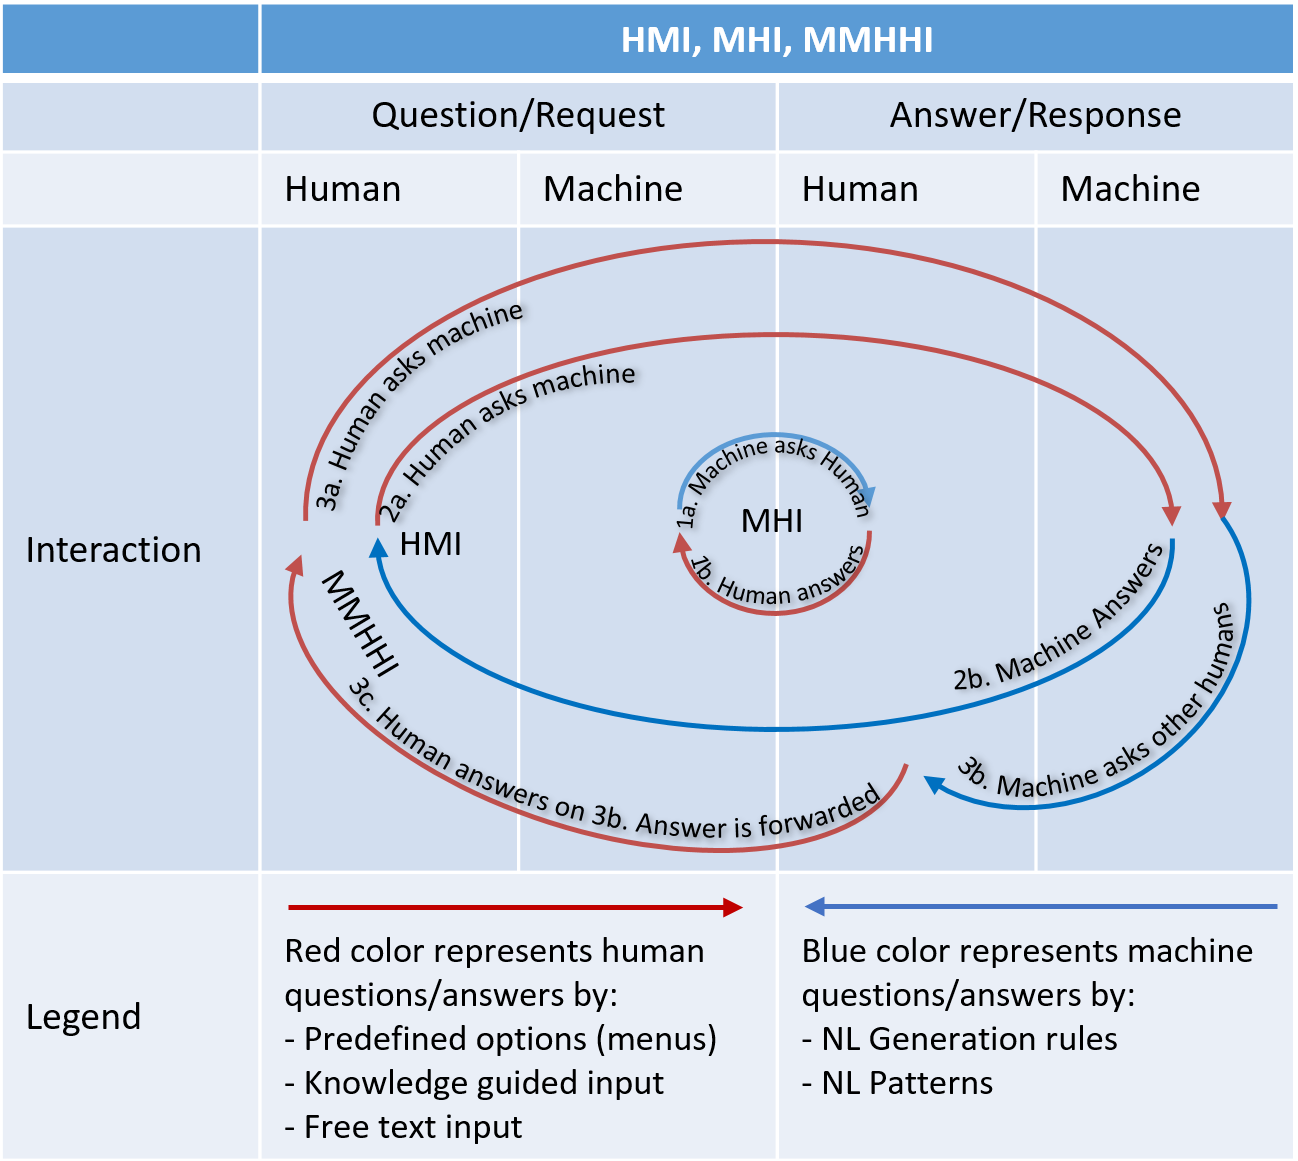
\includegraphics[width=0.9\textwidth]{figures/interactionLoop.png}
	\caption{Possible interaction types between the user and Curious Cat KA
			 System.}
	\label{fig:interaction}
\end{figure}

According to the interactions described above, the proposed KA system have two 
options for the interaction. Human to machine (HMI), when users initiate 
interaction, and machine to human (MHI), when the system initiates the 
interaction. The specifics of both, which cannot fit in 
\autoref{fig:Architecture} are explained in the following sub-sections 
\hl{4.2.1 and 4.2.2}. On top of this, the design of the system allows a novel 
type of interaction which combines multiple users and machine into one 
conversation, while presenting this to the users as a single conversation track
with the machine. This becomes useful when the system doesn't have enough
knowledge to be able to answer user's questions, but it has just enough to know
which other users to ask (i.e. when someone is asking a question about specigic
place and there is no answer in the KB, \emph{Curious Cat} can ask other users
that it knows had been there). This type of the interaction can be called
Machine Mediated Human to Human interaction (MMHHI). This allows the system
to answer questions also when it doesn't know them, while simultaneously also
store and remember the answers, either parsing them and assert them directly to 
KB, or leave them in NL for later Knowledge Mining analysis. The possible
interaction types are also presented on \autoref{fig:interaction}.

\subsubsection{Machine to Human Interaction (MHI)}
\label{section:mhi}
The most basic form of interaction between the CC system and the user, which
we also use the most, is when something triggers a change in the KB and 
CC decides it's the time to ask or tell something. On the 
\autoref{fig:interaction}, this is represented by the most inner loop (MHI). 
Example of this is when the context part of \emph{Procedural} module classifies
a new location and then asserts it into the KB. This then triggers Inference 
Engine which results in a new user query (same as defined in 
\hl{ref to CCWantsToAskLocation}).

\begin{equation*}
	\label{eq:ccWantsLoc}
	ccWantsToAsk(CCUser1, (userLocation(CCUser1,CCLoc1)))
\end{equation*}

This query then goes through logic to NL \hl{ref} conversion, which is then
presented to the user in NL like "Where are we? Are we at the restaurant X?".
This is represented on \autoref{fig:interaction} with a blue arrow on the
inner circle, marked with 1a. The presentation is handled by the client and 
can be in a written form, or through the text-to-speech interface. User can then 
answer this question and thus close the interaction loop (blue arrow marked with
1b), possibly causing a new one with her answer. 

For easier answering, the KA system can use existing KB to generate a set of 
possible answers at the qustion generation time. These can be then picked by
the user instead of writing. THe guidance can consis of variations of these:
\begin{itemize}
	\item A fixed set of pre-defined options that user can pick from, generated
	from the KB.
	\item A set of pre-defined options with an additional free text field when
	the set of possible answers is big or inifite. In this cases the text field
	is connected to the KB providing auto-complete options for valid answers.
	\item Completely free text were user can write anything. This is essentially
	the same as for the HMI interaction described below (\autoref{section:hmi}).
\end{itemize}

The example of mediated answer guidance can be seen in \hl{Fig. 3}, where the 
system presented a set of possible answers while still allowing a free text 
which will be autocompleted with the food types that the system knows about. 
If the user enters something new, the system will accept that (\hl{as was shown 
in the step 6 in Table I)}.

The inference triggering, language rules and mechanisms for context detection
are described in more detail in sections \hl{ref, ref, ref} respectively. This
type of the interaction is where the users answer questions and is thus part of
the main research topic of this thesis.

\subsubsection{Human to Machine Interaction (HMI)}
\label{section:hmi}
The second type of interaction is, when user initiates the conversation. 
If this is done at some point as the answer to an old question, the process is 
the same as described above in \autoref{section:mhi}. But users can also enter a 
free text, asking a question or stating something. In this case, this goes 
through the \emph{NL to Logic Converter} module which tries to convert the
text into logical query or assertion. The complexity of converting NL into logic 
is a lot higher than in the opposite direction, since the language is not
as exact. In CC implementation \hl{ref to CC converter}, we handled this to
some extent by using SCG system \parencite{Schneider2015}, where the text
is matched to NL patterns which are linked to appropriate logical structures.
\hl{This would be used for example, when user, instead of simple Pizza Deluxe 
(step 5 in Table I), would say They sell pizzas or something even more complex 
(see section 4.5.2)}. After the text is converted into logic, inference engine 
can use it to query it against the KB, and show the answers back to user, again 
converted into NL through \emph{Logic to NL Converter} module. This type of
interaction is depicted on \autoref{fig:interaction} by the middle arrow circle
started by humans (arrow 2a), where machine provides the response (arrow 2b).

%SUBSECTION
\subsubsection{Machine Mediated Human to Human Interaction (MMHHI)}
\label{section:mmhhi}
Both of the interactions described in sections \ref{section:mhi} and 
\ref{section:hmi} pre-supposes that the receipient of the query, knows how to
answer it, or respond otherwise. In the cases when, let's say machine doesn't
have any answer (The NL question gets converted into the logical query, which doesn't retrieve any aswers from within the KB). It could respond with 
"I don't know", which is a valid response.
Thile this allows for the conversation to continue, it doesn't help the user
to get the answer, also does not benefit to knowledge acquisition. The only 
thing the system can learn from this, is that user is interested in the object
of the question. This doesn't have to end there though, since CC has access to
other users and knowledge about their past and current contexts. Based on the
topic of interes from the user query, the system can easily find users which
might know the answer (inferred from their past whereabouts, answers, etc.).
Once such an user is deteced, the original question can simply be forwarded to
him, as it would be asked by CC itself. Once he, or one of the users answers,
CC can forward it to the original user. On top of that, CC can parse the answer
the same way as described above for HMI and MHI (sections \ref{section:mhi},
\ref{section:hmi}), and remember it, placing it into the KB. In the cases when
the language of the answer is too complex, it can be stored in its original
format, for later text-mining apporach which can lead to learning of new-patterns
as well as the knowledge hiding in the answers. On top of this, CC can also
remember the question itself, and place it on specific type of concepts, as an
important quetsion to ask. On \autoref{fig:interaction},
MMHHI approach is depicted by the outer circle of arrows, where 3a is original 
user's question, which is forwarded to other users when CC doesn't know how to 
answer (3b). After one or more of the users answer, the answer is forwarded back
to the original user (3c).

%SECTION
\section{Knowledge Base}
\label{section:kb}
As visible in \autoref{fig:Architecture}, Knowledge Base is the central part
of the proposed KA system. Internally KB has three components. The main part, 
which should in any real implementation of the system also be the biggest, is 
the common-sense knowledge, and its upper ontology over which we operate. 
This part of the system contributes the most to the ability to check the 
answers for consistency. The more knowledge already exists, the easier becomes 
to assess the answers, come up with new questions and also propose possible
answers in the guided interaction(\hl{ref}).

The second part is the user Context KB, which stores the contextual knowledge 
about the user. This covers the knowledge that the user has provided about 
himself (\hl{ref}) and the knowledge obtained by mining raw mobile sensors 
(\hl{ref}). On \autoref{fig:Architecture}, This part of the KB is represented 
as the left-most KB, sitting between the main KB and the 
\emph{Procedural Module}.The sensor based context allows the system to 
proactively target the right users at the right time and thus improve the 
efficiency and accuracy and also stickiness of the KA process.

The third KB part, is the meta-knowledge and KA rules that drive the dialog and 
knowledge acquisition process (\hl{ref}). Although in our implementation we 
used Cyc KB (\hl{ref} and also tested Umko KB (\hl{ref}), the approach is not 
fixed to any particular knowledge base. But the KB needs needs to be expressive
enough to be able to cover the intended knowledge acquisition tasks and 
meta-knowledge needed for the system's internal workings. 

Because the full Curious Cat system including the KB is too big and complex to 
be fully explained here (the KA Meta Knowledge alone consists of 12,353 
assertions and rules), we will focus on the fundamentals of the idea and 
approach, and define the simplest possible logic to explain the workings 
through the examples given in the \hl{ref} and  \hl{ref Table II}. 

The logic examples are given in formal higher order predicate logic, which we 
later replace with a more compact notation, with a slight change in the way the 
variables are presented. For better readability, instead of $x, y, z$, we mark 
variables with a question mark ($?$) followed by a name that represents the 
expected type of the concepts the variable represents. For example, when we see 
a variable in a logical formula like $CCUser(?PERSON)$, we immediately know that
$?PERSON$ can be only replaced with (bound to) instance or subclasses of the 
concept $Person$. We start predicate names with a small letter 
($predicate$) and the rest of the 
concepts with a capital letter ($Concept$). At this point it is worth noting 
that while our logical definitions and formalization are strongly influenced by 
Cyc\parencite{Lenat1995}, and while the approach is based on the Cyc upper 
ontology, the approach is general and not bound to any particular 
implementation, and our notation below reflects but is not tightly bound to 
that of OpenCyc. \todo{Add footnotes as in the paper}

%SUBSECTION
\subsection{Upper Ontology}
\label{section:upperOnto}
First we introduce the vocabulary or terms (constants/concepts) that will allow 
us to construct the upper ontology which is the glue of any knowledge base that 
can be used for machine inference:

\begin{equation}\label{set:terms}
\begin{gathered}
S_{Constants} = \{Something, Class, Number, Predicate, subclass, \\
	is, arity, argClass, argIs\}
\end{gathered}
\end{equation}

In the standard \emph{predicate logic}, $P(x)$ notation tells us that whathever 
the $x$ stands for, it has the property defined by the predicate $P$. 
For example, the following propositional function:

\begin{equation}\label{eq:examplepred}
Person(x)
\end{equation}
is stating that something ($x$) is a person, or more precisely, $x$ is an 
instance of a class $Person$. In order to be able to construct logical 
statements ranging
over classes and their instances in a more controlled and transparent way, we
use a constant $is$, and define it as a predicate denoting that something is an
instance of some class.

\begin{definition}[predicate "$is$"]
\label{const:is}
Predicate $is(x,y)$ denotes that $x$ is an instance of $y$. For example, 
stating $is(John, Human)$ defines John as one instance of the class of humans.
\end{definition}
Now, to make things clearer and more precise, instead of writing instance
relation through custom predicate $Person(x)$, we can use more precise syntax, 
which allow us to specify what is instance of which class: $is(x,Person)$.

As visible in the \autoref{eq:examplepred}, in predicate logic, predicates are
defined only with usage. Everything that we write as a predicate in a similar
formula is then defined as a predicate. This is not a desired behavior in our 
KA approach, since the knowledge will be coming from the users with various
backgrounds and without any idea of predicate logic. For this reason we
need more control of what can be used where, if we want to be able to
check for consistencies and have control of our KB with the inference engine.
For this reason, we enforce a constraint (rule).

\begin{definition}[Predicate Constraint]\label{constraint:predicate}
Everything that we want to use in the KB as a predicate, must first be defined
as an instance of the $Predicate$ class:
$\forall x \in S_{Predicates}: is(x,Predicate)$. From the other side, set of
predicates can be defined as $S_{Predicates}=\{x:is(x,Predicate)\}$.
This constraint can be inserted into our KB as a \emph{material implication}
rule, which needs to be true at all times, to serve as a constraint:
\begin{equation}\label{rule:pred_constraint}
\forall P \forall x_{1...n} (P(x_1...x_n) \implies is(P,Predicate))
\end{equation}
\end{definition}

Now, careful reader might notice, that we actually cannot use $is$ as a 
predicate, since nowhere in our KB is stated that this is actually a 
predicate. To fix this error and make our KB consistent with its constraints,
we need to add an assertion defining what term $is$ stands for:

\begin{equation}\label{as:is_is}
is(is, Predicate)
\end{equation}
At the time the above assertion (Assertion \ref{as:is_is}) is asserted
into the KB, it also becomes valid assertion, since it complies with the
constraint defined in Definition \autoref{constraint:predicate} and thus our
Constraint Rule \ref{rule:pred_constraint} is true. After this 
assertion is in the KB, $ir$ can be used as a predicate because it is an 
instance of the term $Predicate$ and complies with our constraints. 

At this point we can define(assert) the rest of our predicates:

\begin{equation}\label{as:predicates}
\begin{gathered}
is(subclass, Predicate) \land is(arity,Predicate) \land is(argClass,Predicate)\\
\land is(argIs,Predicate)
\end {gathered}
\end{equation}
And also the rest of our terms, which we define as instances of term $Class$.
\begin{equation}\label{as:is_class}
\begin{gathered}
	is(Class,Class) \land is(Predicate,Class)\\ 
\land is(Number, Class)
\end {gathered}
\end{equation}

In Predicate logic, predicates have a property called arity, which defines 
number of arguments that the predicate can have. For example, if predicate
$P$ has arity of 1, then it can only take one operand (variable or term). In 
this case only $P(x)$ or $P(a)$ are valid statements, and $P(x,y)$ is not.
In our KB, arity is defined using $arity$ predicate, which itself was defined
in Assertion \ref{as:predicates}.

\begin{definition}[predicate "$arity$"]\label{def:arity}
Predicate $arity(x,y)$ denotes that predicate $x$ has arity of $y$.
\end{definition}

Similarly, as with the constraint that all predicates need to be defined as
such (Definition \autoref{constraint:predicate}), we gain more control over 
KB and make things easier for the inference engine and KA approach, if we 
limit the assertions, to "obey" the predicate arities. For this reason our KB
has additional constraint.

\begin{definition}[Arity Constraint]\label{constraint:arity}
All assertions in CC KB are valid only, when the predicates used in the 
assertion have the same number of arguments as defined with their $arity$ 
assertions:
\begin{equation}\label{rule:arity_constraint}
\forall P \forall n \forall x_{1...n}:(P(x_1,...,x_n) \implies arity(P,n))
\end{equation}
\end{definition}

After we add the above rule (Constraint Rule \ref{rule:arity_constraint}), our 
KB is not consistant anymore, since all the $is(x,y)$ assertions (Assertions 
\ref{as:is_is}, \ref{as:predicates}) violate the constraint. We fix this by 
adding the following assertion:

\begin{equation}\label{as:arity_is}
arity(arity,2) \land arity(is,2)
\end{equation}
This makes the KB consistant again, because we defined all the arities of
predicates $arity$ and $is$, which we have used so far in our KB, as well as 
defined them with $is(x, Predicate)$ assertions. We can now continue with 
defining the arities of the rest of the predicates:

\begin{equation}\label{as:arity_predicates}
\begin{gathered}
arity(subclass, 2) \land arity(argClass,3) \land arity(argIs,3)
\end {gathered}
\end{equation}
We can see now that the arity of $is$ predicate is defined as 2 (same as for 
$subclass$ and $arity$, which can be used to define arity of itself), and can 
confirm that all the logical formulas in the definitions up to now are correct.

To be able to describe the world in more detail, we define the $subclass$ 
predicate, which handles the hierarchy relations between multiple classes 
(unlike $is$, which handles relationships between classes and their instances).

\begin{definition}[predicate "$subclass$"]\label{def:pred_subclass}
Predicate $sublcass(x,y)$ denotes that $x$ is a subclass of $y$. For example, 
asserting $subclass(Dog, Animal)$, is specifying all dogs, to be a sub-class of
animals, and $subclass(Terrier,Dog)$ is speficfying that all terriers are 
sub-class of dogs. At this point we might notice that while it is logical to us
that terriers are also a sub-class of animals, there is no way for the machine
inference to figure that out. For this reason we need to introduce a
"subclass transitivity" inference rule:
\begin{equation}\label{rule:subclass_transitivity}
\begin{gathered}
  \forall x \forall y \forall z: ((subclass(x,y) \land subclass(y,z)) \implies subclass(x,z))
\end{gathered}
\end{equation}
The rule above is basically saying that if a first thing is a sub-class of a
the second thing, and then thesecond thing is a subclass of the thirdthing,
then the third thing is a sub-class of the first thing as well. 
\end{definition}

Because we want to be able to prevet our system from acquiring incorrect 
knowledge, we need to limit the domains and ranges of the predicates 
(arguments). This could be done by adding a speciic constraint rules
(material implication rule without the power to make new assertions). For 
example, for both $subclass$ arguments, to only allow instances of a $Class$, 
we could assert:
\begin{equation}\label{as:domain_example}
  \forall x_1 \forall x_2: (subclass(x_1,x_2) \implies (is(x_1,Class) \land 
  is(x_2,Class))
\end{equation}
Because the rule (Rule \ref{as:domain_example} is only true if the right part
(the consequent) is true, or the left part (the antecedent) is false, its
inclusion in the KB (as with other constraint rules) forces the KB to not allow
the arguments of subclass to be anything else than an instance of a class 
$Class$. It would be hard to construct a large KB, by writing the rule
like this for each of the thousands potential predicates. To make this easier,
following Cyc practice\parencite{Lenat1995}, we will introduce $argIs$ 
predicate (Definition \ref{def:pred_subclass}). To make this definition more understandable, let's
first expand the example (Rule \ref{as:domain_example} above:

\begin{equation}\label{as:domain_ext_example}
\begin{gathered}
  \forall x_1 \forall x_2: (subclass(x_1,x_2) \implies (is(x_1,Class) \land is(x_2,Class)) \\ 
  \iff \\
  argIs(subclass,1,Class) \land argIs(subclass,2,Class))
\end{gathered}
\end{equation}
This rule above (Rule \ref{as:domain_ext_example} states, that the constraint
rule (Rule \ref{as:domain_example} can be written as 2 $argIs$ assertions.
Instead of writing full rule, the constraint for the argunent of $subclass$ can
be written simply as $argIs(subclass,1,Class)$. To make this hold for all the
combinations of predicates (not just $subclass$ from example), we can
re-phrase the rule to be general, and also define the $argIs$ predicate.

\begin{definition}[predicate "$argIs$"]\label{def:pred_argis}
Predicate argIs(x,y,z) denotes that the $y-th$ argument of predicate $x$, must
be an instance of $z$. For example, asserting \\$argIs(subclass,1, Class)$, states
that the first argument of predicate $subclass$ must be an instance of $Class$.
This is enforced by the following constraint rule:
\begin{equation}\label{as:domain_isa_constraint}
\begin{gathered}
  \forall P \forall n \forall x_1...x_n \forall C_{1...m}: \\
  ((arity(P,n) \land P(x_1,...,x_n)) \implies (is(x_1,C_{1...m}) \land ... \land is(x_n,C_{1...m})) \\ 
  \iff \\
  argIs(P,1,C_{1...m}) \land ... \land argIs(P,n,C_{1...m}))
\end{gathered}
\end{equation}
\end{definition}

These definitions allow us to use simple $argIs$ assertions, instead of
complicated rules. For the cases, when the arguments shouldn't be instances
of a $Class$, but its subclasses, we can define similar predicate and its
constraint rules also fro $argClass$:

\begin{definition}[predicate "$argClass$"]\label{def:pred_argClass}
Predicate $argClass(x,y,z)$ denotes that the $y-th$ argument of predicate $x$, 
must be a subclass of $z$. For example, asserting 
\\$argClass(servesCuisine, 2, Restaurant)$, states that the first argument of 
predicate $servesCuisine$ must be a subclass of $Restaurant$.
This is enforced by the following constraint rule (similar as for $argIsa$, but
for $argClass$):
\begin{equation}\label{as:domain_class_constraint}
\begin{gathered}
  \forall P \forall n \forall x_1...x_n \forall C_{1...m}: \\
  ((arity(P,n) \land P(x_1,...,x_n)) \implies (subclass(x_1,C_{1...m}) \land ... \land subclass(x_n,C_{1...m})) \\ 
  \iff \\
  argClass(P,1,C_{1...m}) \land ... \land argClass(P,n,C_{1...m}))
\end{gathered}
\end{equation}
\end{definition}

Before we can assign argument constraints to our existing predicates and have
all the KB valid, we need to define a special class $Number$:

\begin{definition}[class $Number$ and its instances]\label{def:number}
All natural numbers are instances of the class $Number$. Formally, this can be
asserted into a KB as:
\begin{equation}\label{as:numbers}
	\forall x \in \mathbb{N}:is(x,Number)
\end{equation}
\end{definition}

This now allows us to use $argIs$ and $argClass$ predicates instead of 
complicated rules, to define types of arguments inside any predicate used in the
KB. By using these two newly defined predicates, we can now proceeed to assert 
the argument limits of the $argIsa$ predicate itself: 

\begin{equation}\label{as:argIs_domain}
\begin{gathered}
argIs(argIs,1,Predicate) \land argIs(argIs,2,Number) \land argIs(argIs,3,Class) 
\end{gathered}
\end{equation}
We can see that the first argument must be an instance of $Predicate$, which 
holds in all three cases ($argIs$ is a first argument of the Assertion 
\ref{as:argIs_domain} above), since it was defined in Assertion 
\ref{as:predicates}. Similary, the second argument is a valid number, in all 
three cases as defined in Definition \ref{def:number}. Also the third arguments
($Predicate$, $Number$,$Class$), are all instances of the $Class$ as defined in
Assertion \ref{as:is_class}, so the assertion \ref{as:argIs_domain} can be asserted
and it doesn't invalidate itself throigh argument contraint rule (Constraint 
\ref{as:domain_isa_constraint}).

Similary, we can now proceed to define the rest of our predicates. Starting with
the most similar $argClass$:
\begin{equation}\label{as:argClass_domain}
\begin{gathered}
	argIs(argClass,1,Predicate) \land argIs(argClass,2,Number) \\
	\land argIs(argClass,3,Class) 
\end{gathered}
\end{equation}
Since we didn't yet assert any direct $argClass$ constraint, this predicate
at this point defines the constraints, without any danger to invalidate our
current KB. 

Continuing with $subclass$. On the Definition \ref{def:pred_subclass}, 
we can see that this
predicate defines sub-class relationships between the classes. For this reason
it makes sense to only allow instances of $Class$ for its arguments:
\begin{equation}\label{as:subclass_is_constraint}
	argIs(subclass,1,Class) \land argIs(subclass,2,Class)
\end{equation}
Same as with the Assertion \ref{as:argClass_domain}, we didn't yet assert any 
direct assertions about something being a sub-class of something, this assertion
doesn't affect yet the validity of our KB, while prevents future assertions of 
$subclass$ predicate on anything but $Class$ instances.

For the $arity$ predicate, we can check our existing assertions 
(\ref{as:arity_is}, \ref{as:arity_predicates}), and
see that as the first argument we always have an instance of $Predicate$, while
as the second argument we have an instance of a $Number$. According to this, it
serves our purpose and is safe to limit the arguments of $arity$ to:
\begin{equation}\label{as:arity_is_constraint}
	argIs(arity,1,Predicate) \land argIs(arity,2,Number)
\end{equation}

We can now proceed to define our last ($is$) predicate constraints, which is
a bit more complicated. If we look at our existing  $is$ assertions 
(\ref{as:is_is}, \ref{as:predicates}, \ref{as:numbers}), we can
see that as a second argument we always have an instance of a $Class$ 
($Predicate$, $Class$), but
for the first argument we can actually put in anything ($is$, $Class$, 
$Predicate$,  $Number$, $\mathbb{N}$). From instance of a $Class$,
instance of a $Predicate$, to an instance of a $Number$. For the second argument
we can imediatelly asert

\begin{equation}\label{as:is_arg2_domain}
argIs(is,2, Class)
\end{equation}

In order to be able to say that some argument can be anything, we followed a 
Cyc example and introduce term $Something$, first mentioned in the set of our 
terms in Assertion \ref{set:terms}. We set this as the constraint for the first
argument of $is$ predicate:

\begin{equation}\label{as:is_arg1_domain}
argIs(is,1, Something)
\end{equation}
But this assertion above (\ref{as:is_arg1_domain}), invalidates the correctnes
of all of our $is$ assertions, since none of the current first arguments are
instances o $Something$ (see Assertions \ref{as:is_is}, \ref{as:predicates} and 
\ref{as:numbers}). To fix this, we need to be able at least to say that things 
are instances of $Something$ ($is(x,Something)$). According to the $is$ argument
constraint assertion above (\ref{as:is_arg2_domain}), $Something$ must be an 
instance of a $Class$. So we define it as so:

\begin{equation}\label{as:is_something}
	is(Something,Class)
\end{equation}
Now, as a consequence of this, we could assert for all of the arguments that
are used in $is$ ($is$, $Class$, $Predicate$, $Number$, $\mathbb{N}$), that 
they are an instances of the $Something$. This would
be highly unpractical, since we would need to do this for every future constant
to be used by $is$ predicate (especially unpractical for infinite number of
$\mathbb{N}$).

Instead, since we know that $Something$ is an instance of a $Class$, we can use 
it in our $subclass$ assertions (a consequence of constraint Assertion 
\ref{as:subclass_is_constraint}) and state that $Class$ is a subclass of 
$Something$:
\begin{equation}\label{as:subclass_something}
	subclass(Class, Something)
\end{equation}
A consequence of this assertion is (because of inference rule 
\ref{rule:subclass_transitivity}), that
every sub-class of anything that exists in our KB (because we can only use 
instances of $Class$ in $subclass$ assertions), is a sub-class of $Something$ as
well. This doesn't yet seem to help us make our 1st $is$ predicate arguments 
instances of $Something$, but it will, after we address another weaknes in our
current KB. 
Consider the continuation of the example we started in $subclass$ 
definition (Definition \ref{def:pred_subclass}, where a terrier is a sub-class
of dog, and dog is a sub-class of animals ($subclass(Dog,Animal)$, 
$subclass(Terrier,Dog)$). If we introduce an instance of the
class $Terrier$, let's say, a real dog named "Spot" ($is(Spot,Terrier$)), we can
see that there is a logical problem, since Spot is a terrier in our KB, but
not a dog, or even an animal (there is nothing to support $is(Spot,Animal)$ 
assertion. This can be fixed by introducing the following Inference Rule:

\begin{equation}\label{rule:is_transfer}
\begin{gathered}
  \forall x \forall y \forall z: ((is(x,y) \land subclass(y,z)) \implies is(x,z))
\end{gathered} \end{equation}
This rule is basically saying, that if there is an instance of a class, and this
class is a sub-class of another class, then this instance is also an instance of
the other class. Now, this inference rule (\ref{rule:is_transfer}), together 
with the fact that $Class$ is a sub-class of $Something$, and the $subclass$
transitivity inference rule (\ref{rule:subclass_transitivity}), makes everything
 that is instance of a 
class, or its sub-class (which is everything in our KB), also an instance of
$Something$, and thus proving the assertion \ref{as:is_arg1_domain} correct and 
consequently our KB fully consistant again.

At this point our Upper Ontology is defined (it is visually presented on
\autoref{fig:upperOnto}) and ready to build upon as will be
described in the next chapters. Since Curious Cat main implementation is based
on Cyc, and it was inspired by the way Cyc ontology is constructed and being 
used, this upper ontology reflects the main part of Cyc upper ontology 
(see Chapter \ref{chapter:implementation}, implementation on how this 
formalization maps to Cyc). While our upper ontology logical definitions and 
formalizations are strongly influenced by Cyc, the approach is general and not 
bound to any particular implementation, and our notation reflects but is not 
tightly bound to that of Cyc. For example, the usage of $argIs$ and $argClass$
can be replaced by $domain$ and $range$ when using a RDF schema, such as was 
done in our RDF prototype implenentation\parencite{Bradesko2012a}, or a 
completely custom constraints can be used in specific ontologies, so this
upper ontology is more of a guidence and a tool to be able to explain apporach,
than a fixed ontology that needs to be implemented.

\begin{figure}[H]
	\centering
		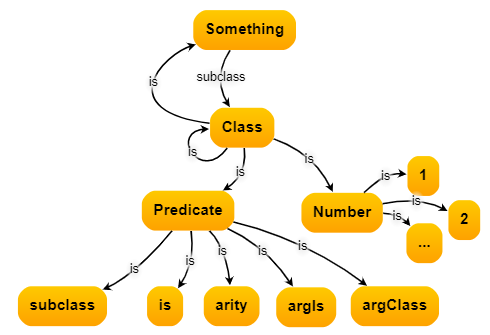
\includegraphics[width=0.8\textwidth]{figures/upperOntology.png}
	\caption{Upper ontology terms, with 'is' and 'subclass' relations.}
	\label{fig:upperOnto}
\end{figure}

%SUBSECTION
\subsection{Existing Knowledge}
\label{section:existingKB}
This sub-chapter extends our upper ontology example with additional knowledge
that allows us to explain the system through the examples given in 
\autoref{tab:conversation1} and \autoref{tab:conversation2}. 

As also visible in the Architecture schematic (\autoref{fig:architecture},
KB with background knowledge is one of the most crucial elements of proposed 
approach. It serves both, as the driving force behind the source of the 
questions, since with the help of contextual knowledge triggers the infrence to
produce logical queries for the missing parts of the knowledge. At the same time
it is the drive behind the proactive user interaction, sarting either as a
question or a suggestion. Finally, the background knowledge is also used for 
validation of answered questions. If the answers are not consistent according
to the existing KB, users are required to re-formulate, or repeat the answer.

The main \emph{Curious Cat} implementation, uses an extended 
full Cyc ontology and KB, similar to that released as ResearchCyc, as a 
common sense and background knowledge base. This is far too big (millions of 
assertions), to be explained in any detail here with the general approach (it 
is explained in more detail in Chapter \ref{chapter:implementation}, 
Implementation). In this chapter we define only the concepts and predicates 
and thus construct the minimal example KB that is necessary for explaining the p
roposed system.

First we introduce the set of new concepts that we need for the food part
of the ontology. These concepts are defined on top of the existing Upper 
Ontology, so the new parts of the KB should maintain the consistency of the
already described parts. The set of terms $S_{Food} $, needed to describe this 
part of the KB is as follows:

\begin{equation}\label{set:foodTerms}
\begin{gathered}
S_{Food} = \{FoodOrDrink,Food,Bread,Baguette,Drink,Coffee\}
\end{gathered}
\end{equation}
Where each of these terms is an instance of a $Class$:
\begin{equation}\label{set:foodTermsClass}
\begin{gathered}
\forall x \in S_{Food}: isa(x,Class)
\end{gathered}
\end{equation}
Then, these classes are connected into a class-hierarchy, which is done with
a $subclass$ predicate:

\begin{equation}\label{as:kbFoodSubclasses}
\begin{gathered}
    subclass(Drink,FoodOrDrink) \land subclass(Coffee,Drink) \land \\
	subclass(Food,FoodOrDrink) \land subclass(Bread,Food) \land \\
	subclass(Baguete, Bread)
\end{gathered}
\end{equation}
Which is also presented graphically on \autoref{fig:foodSubclass} below.
\begin{figure}[H]
	\centering
		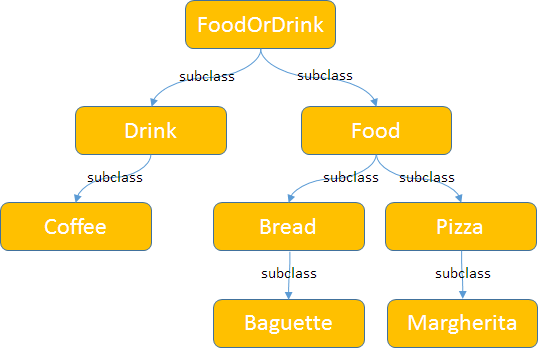
\includegraphics[width=0.6\textwidth]{figures/foodOntology.png}
	\caption{Hierarchy of food related terms, specified by subclass predicates.}
	\label{fig:foodSubclass}
\end{figure}

The second part of ontology (KB) constructing knowledge about places consist
of the following terms:

\begin{equation}\label{set:placeTerms}
\begin{gathered}
S_{Place} = \{Placa,PublicPlace,PrivatePlace,Restaurant\}
\end{gathered}
\end{equation}
Where each of these terms is also an instance of a $Class$:
\begin{equation}\label{set:placeTermsClass}
\begin{gathered}
\forall x \in S_{Place}: isa(x,Class)
\end{gathered}
\end{equation}
Then, these classes are connected into a class-hierarchy, which is done with
a $subclass$ predicate:

\begin{equation}\label{as:kbPlaceSubclasses}
\begin{gathered}
    subclass(PrivatePlace,Place) \land subclass(PublicPlace,Place) \land \\
	subclass(Restaurant,PublicPlace) \land subclass(Home,PrivatePlace)
\end{gathered}
\end{equation}
And, in order to have some "real-world" knowledge, we also add an example 
instance of a real restaurant represented as term $Restaurant1$.
\begin{equation}\label{as:restaurant1}
	is(Restaurant1,Restaurant)
\end{equation}
This is all presented graphically on \autoref{fig:placeOntology} below.
\begin{figure}[H]
	\centering
		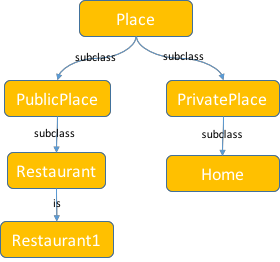
\includegraphics[width=0.5\textwidth]{figures/placeOntology.png}
	\caption{Hierarchy of place related terms, specified by subclass predicates.}
	\label{fig:placeOntology}
\end{figure}

Then the last part (excluding predicates which are defined separately),
of our \emph{Existing Knowledge} consist of the following terms:

\begin{equation}\label{set:otherTerms}
\begin{gathered}
S_{Reest} = \{Service,WirelessService,Vehicle,Car,Animal,Duck,\\
	Human,User\}
\end{gathered}
\end{equation}
Where each of these terms is also an instance of a $Class$:
\begin{equation}\label{set:restTermsClass}
\begin{gathered}
\forall x \in S_{Rest}: isa(x,Class)
\end{gathered}
\end{equation}
And a class-hierarchy:

\begin{equation}\label{as:kbPlaceSubclasses}
\begin{gathered}
    subclass(Car,Vehicle) \land subclass(WirelessService,Service)\land\\
	subclass(Duck,Animal)\land subclass(Human,Animal)\land \\
	subclass(User,Human)
\end{gathered}
\end{equation}
And an instance of the $User$ class representing one CC user.
\begin{equation}
	is(User1,User)
\end{equation}

Which is also presented graphically on \autoref{fig:restOntology} below.
\begin{figure}[H]
	\centering
		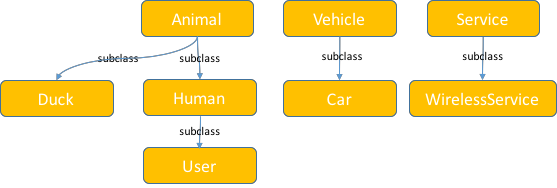
\includegraphics[width=0.9\textwidth]{figures/restOntology.png}
	\caption{Hierarchy of the rest of the terms from our \emph{existing 
	knowledge.}}
	\label{fig:restOntology}
\end{figure}
We can see that all these new terms add on top of the existing set of terms from 
upper ontology ($S_{Constants} = S_{upper} \cup S_{Food} \cup S_{Place} 
\cup S_{Rest}$). 

For defining the predicates, we need a bit more detailed definitions, since we 
also want to represent the constraints which will serve for the inference 
engine to check the validity of the answers (as explained in 
\hl{ref to constraints def. in UpperOnto}).

\begin{definition}[predicate $menuItem$]\label{def:menuItem}
Predicate $menuItem(x,y)$ denotes that place $x$ has a menu item $y$ on its 
menu.Formally it is defined as:
\begin{equation}\label{as:pred_menuItem}
\begin{gathered}
    is(menuItem,Predicate) \land \\
	argIs(menuItem,1,Restaurant) \land\\
	argClass(menuItem,2,FoodOrDrink)
\end{gathered}
\end{equation}
\end{definition}
As we see defined above (assertion \ref{as:pred_menuItem}), this predicate
constraints allow us to only use instances of class $Restaurant$ for the first
argument, and sub-classes of class $FoodOrDrink$ for the second. Example of this
is the following assertion that we use to have an example restauratn instance
in our KB (to continue the definition of Assertion \ref{as:restaurant1}), saying
that Restaurant1 has coffee on the menu:
\begin{equation}
menuItem(Restaurant1,Coffee)
\end{equation}

Besides the 
items on the menu, to explain our examples, we also need a way to tell that
a place provides some services.

\begin{definition}[predicate $providesServiceType$]\label{def:serviceType}
Predicate $providesServiceType(x,y)$ denotes that place $x$ provides service 
$y$. Formally it is defined as:
\begin{equation}\label{as:providesServiceType}
\begin{gathered}
    is(providesServiceType,Predicate) \land \\
	argIs(providesServiceType,1,Place) \land\\
	argClass(providesServiceType,2, Service)
\end{gathered}
\end{equation}
\end{definition}
As defined in the Assertion \ref{as:providesServiceType}, $providesServiceType$
constraints allow us to only use instances of class $Place$ (Public,Private,
Home,Restaurant for the current stage of the KB) for the first argument, and 
sub-classes of class $Service$ for the second. 

\begin{definition}[predicate $userLocation$]\label{def:userLocation}
Predicate $userLocation(x,y)$ denotes that user $x$ is located at place 
$y$. Formally it is defined as:
\begin{equation}\label{as:userLocation}
\begin{gathered}
    is(userLocation,Predicate) \land \\
	argIs(userLocation,1,User) \land\\
	argIs(userLocation,2, Place)
\end{gathered}
\end{equation}
\end{definition}
As defined in the Assertion \ref{as:userLocation}, $userLocation$
constraints allow us to only use instances of class $User$ for the first
argument, and instances of $Place$ as a second.

\begin{figure}[H]
	\centering
		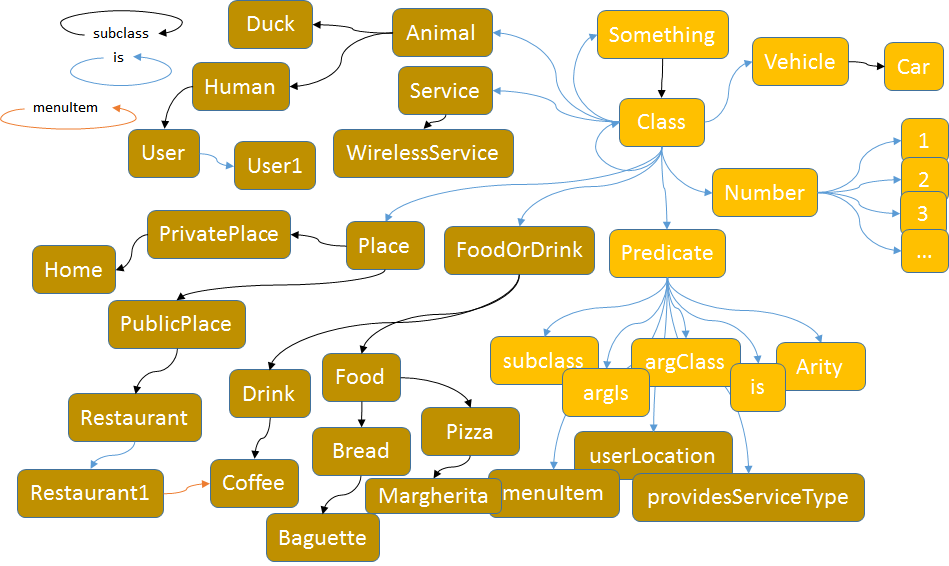
\includegraphics[width=1\textwidth]{figures/fullExistingKB.png}
	\caption{Current "existing knowledge" on top of upper ontology}
	\label{fig:existingKB}
\end{figure}

At this point we have a formal KB structure representing a minimal 
\emph{existing knowledge} required to explan the examples from 
\autoref{tab:conversation1} and \autoref{tab:conversation2}. The KB is
graphically presented on the \autoref{fig:existingKB}, where the upper ontology
is presented in lighter color and new KB parts in darker. Due to lack of space,
the only relations are of $is$ (represented by blue arrows), $subclass$ 
(represented with black arrows) and $menuItem$ (orange arrow) predicates.

%SUBSECTION
\subsection{KA Knowledge}
\label{section:kakb}
In the previous two sections we defined the upper ontology
(Section \ref{section:upperOnto}) and then using its vocabulary to define the 
pre-existing knowledge (Section \ref{section:existingKB}). This will suffice to
support the explanation of the proposed KA approach. Similar as with the other
parts of the KB, listing full set of 
\emph{Curious Cat} KA rules would not fit in the paper. Instead we define an 
example set of the KB, sufficient for describing the approach and keeping the 
explanation as simple as possible. 

As a starting point, we need to define a main KA meta-class $Formula$, which’s 
is a special class (like $Number$).
\begin{definition}[class $Formula$ and its instances]\label{def:formula}
All logical formulas (assertions, queries) are instances of the class $Formula$.
Formally, this can be represented as:
\begin{equation}\label{as:formulas}
\begin{gathered}
	\forall P\forall x_{1...n}:is(P(x_1,...,x_n),Formula)
\end{gathered}
\end{equation}
Basically all of the content of the KB and queries are instances of $Formula$.
For example, assertion $userLocation(User1,Ljubljana)$ is an instance of 
$Formula$ and consequentially the statement $is(userLocation(User1,Ljubljana),
Formula)$ is true.
\end{definition}

Then we need to define additional KA meta predicates:

\begin{definition}[predicate "$known$"]\label{def:pred_known}
Special meta-predicate $known(x)$ denotes that the formula $x$ can be proven 
in the KB. This predicate is non-assertible, meaning that it cannot be used
to add things into the KB, but it can be used in inference rules. For example,
since the Assertion \ref{as:is_something} is already asserted in the KB and 
true, the query/un-assertible statement $known(is(Something,Class))$ is also 
true. The predicate is formally defined as follows:
\begin{equation}\label{as:known}
\begin{gathered}
	is(known,Predicate) \land arity(known,1) \land argIs(known,1,Formula)
\end{gathered}
\end{equation}
\end{definition}

In a similar fashion as predicate $known$, we define $unknown$ predicate.

\begin{definition}[predicate "$unkknown$"]\label{def:pred_unknown}
Special meta-predicate $unknown(x)$ denotes that the formula $x$ can 
\textbf{not} be proven in the KB. This predicate is non-assertible, meaning that it cannot be used to add things into the KB, but it can be used in inference 
rules. Building on the example given in the Definition \ref{def:pred_known}
($known$ predicate), the query $unkown(is(Something,Class))$ is 
\textbf{not true}, since the assertion exist an is known. On the other hand,
$unknown(is(Human,Duck))$ is true, since there is no knowledge in the KB which
would support the encapsulated $is$ statement. The predicate is formally defined as follows:
\begin{equation}\label{as:unknown}
\begin{gathered}
	is(unknown,Predicate) \land arity(unknown,1) \land argIs(unknown,1,Formula)
\end{gathered}
\end{equation}
\end{definition}

And now one of the main KA predicates, which is used to provide the CC system
with the formulas which need to be converted to NL and presented to the user.
\begin{definition}[predicate "$ccWantsToAsk$"]\label{def:pred_ccWantsToAsk}
One of the main KA predicates written as $ccWantsToAsk(x,y)$, denotes that the 
\emph{Curious Cat} system wants to ask user $x$ a question represented by the
formula $y$. For example, assertion 
\begin{equation*}
ccWantsToAsk(User1, userLocation(User1,x))
\end{equation*}
tells CC system to ask user the question $userLocation(User1,x)$, which,
after it goes through logic to NL conversion \hl{ref} is paraphrased as
"Where are we?", as hinted in the step \ref{step:where} in the 
\autoref{tab:conversation1}. The predicate is formally defined as follows:
\begin{equation}\label{as:ccWantsToAsk}
\begin{gathered}
	is(ccWantsToAsk,Predicate) \land arity(ccWantsToAsk,2) \land\\ 
	argIs(ccWantsToAsk,1,User) \land argIs(ccWantsToAsk,2,Formula)
\end{gathered}
\end{equation}
\end{definition}

Now, after we have supporting predicates, we can define an example of KA rule, 
KA rules can written specifically to enable the production of questions for a 
narrow context, or generally, covering broad scope of questions as the
following:

\begin{equation}\label{as:generalRule}
\begin{gathered}
\forall i_1 \forall c \forall i_2 \exists s_2 \forall u:is(i_1,c) \land P(i_1,s) \land is(i_2,c)\land unknown(P(i_2,s_2)) \\ 
	\implies \\
ccWantsToAsk(u,P(i_2,\$x))
\end{gathered}
\end{equation}
This rather complicated material implication causes generation of question 
intents whenever there is an instance of a class that was used in an arity 2 
predicate, and there is another instance of the same class which doesn’t have 
any assertion using this predicate. When the antecedent of this rule is true,
then the consequent is a $ccWantsToAsk$ predicate representing an open
ended logical query (NL question) asking for the things that can fullfill the
predicate $P$ for instances of aforementioned class. \hl{maybe add/explain
list of suggestions as well}.

If we take our example KB (\autoref{fig:existingKB}) and imagine we assert
an additional instance of a $Restaurant$ (Restaurant2: "Joe’s Pizza", as was 
done in the example conversation in \autoref{tab:conversation1}, 
step \ref{step:where}, the premises of the rule can get satisfied like this:
\begin{equation}\label{as:generalRuleantecedent}
\begin{gathered}
is(Restaurant1,Restaurant) \land menuItem(Restaurant1,Coffee)\land \\
	is(JoesPizza,Restaurant) \land unknown(\exists s_2:menuItem(JoesPizza,s_2))
\end{gathered}
\end{equation}
Because all of the above premises are true, including the $unknown$ part
(there is no support in the KB for the formula inside $unknown$ predicate - see 
Definition \hl{def for unknown}), this rule in our KB up to now produces the 
following consequent:
\begin{equation}\label{as:generalRuleConsequent}
\begin{gathered}
	ccWantsToAsk(User1,menuItem(JoesPizza,x))
\end{gathered}
\end{equation}
representing an intent of CC system to ask user the question 
$menuItem(JoesPizza,x)$, which converted to NL comes out as "What is on the menu
in Joe's Pizza", which matches the step \ref{step:menu} from the \autoref{tab:conversation1}.

B\hl{Emphasise how \$x got transferred, tehn continue with the explanation}

% SUBCHAPTER
\subsection{Context}
\begin{definition}[predicate "$probableUserLocation$"]
\label{pred:probableUserLocation}
Dada\hl{Maybe define this one at the end, since it could also be defined in the
Context section}
\end{definition}
